% Options for packages loaded elsewhere
\PassOptionsToPackage{unicode}{hyperref}
\PassOptionsToPackage{hyphens}{url}
%
\documentclass[
]{book}
\usepackage{amsmath,amssymb}
\usepackage{lmodern}
\usepackage{iftex}
\ifPDFTeX
  \usepackage[T1]{fontenc}
  \usepackage[utf8]{inputenc}
  \usepackage{textcomp} % provide euro and other symbols
\else % if luatex or xetex
  \usepackage{unicode-math}
  \defaultfontfeatures{Scale=MatchLowercase}
  \defaultfontfeatures[\rmfamily]{Ligatures=TeX,Scale=1}
\fi
% Use upquote if available, for straight quotes in verbatim environments
\IfFileExists{upquote.sty}{\usepackage{upquote}}{}
\IfFileExists{microtype.sty}{% use microtype if available
  \usepackage[]{microtype}
  \UseMicrotypeSet[protrusion]{basicmath} % disable protrusion for tt fonts
}{}
\makeatletter
\@ifundefined{KOMAClassName}{% if non-KOMA class
  \IfFileExists{parskip.sty}{%
    \usepackage{parskip}
  }{% else
    \setlength{\parindent}{0pt}
    \setlength{\parskip}{6pt plus 2pt minus 1pt}}
}{% if KOMA class
  \KOMAoptions{parskip=half}}
\makeatother
\usepackage{xcolor}
\usepackage{longtable,booktabs,array}
\usepackage{calc} % for calculating minipage widths
% Correct order of tables after \paragraph or \subparagraph
\usepackage{etoolbox}
\makeatletter
\patchcmd\longtable{\par}{\if@noskipsec\mbox{}\fi\par}{}{}
\makeatother
% Allow footnotes in longtable head/foot
\IfFileExists{footnotehyper.sty}{\usepackage{footnotehyper}}{\usepackage{footnote}}
\makesavenoteenv{longtable}
\usepackage{graphicx}
\makeatletter
\def\maxwidth{\ifdim\Gin@nat@width>\linewidth\linewidth\else\Gin@nat@width\fi}
\def\maxheight{\ifdim\Gin@nat@height>\textheight\textheight\else\Gin@nat@height\fi}
\makeatother
% Scale images if necessary, so that they will not overflow the page
% margins by default, and it is still possible to overwrite the defaults
% using explicit options in \includegraphics[width, height, ...]{}
\setkeys{Gin}{width=\maxwidth,height=\maxheight,keepaspectratio}
% Set default figure placement to htbp
\makeatletter
\def\fps@figure{htbp}
\makeatother
\setlength{\emergencystretch}{3em} % prevent overfull lines
\providecommand{\tightlist}{%
  \setlength{\itemsep}{0pt}\setlength{\parskip}{0pt}}
\setcounter{secnumdepth}{5}
\usepackage{booktabs}
\usepackage{amsthm}
\makeatletter
\def\thm@space@setup{%
  \thm@preskip=8pt plus 2pt minus 4pt
  \thm@postskip=\thm@preskip
}
\makeatother
\ifLuaTeX
  \usepackage{selnolig}  % disable illegal ligatures
\fi
\usepackage[]{natbib}
\bibliographystyle{apalike}
\IfFileExists{bookmark.sty}{\usepackage{bookmark}}{\usepackage{hyperref}}
\IfFileExists{xurl.sty}{\usepackage{xurl}}{} % add URL line breaks if available
\urlstyle{same} % disable monospaced font for URLs
\hypersetup{
  pdftitle={(Otro) Manual de metodología de la investigación en ciencias sociales},
  pdfauthor={Lucas Sempé},
  hidelinks,
  pdfcreator={LaTeX via pandoc}}

\title{(Otro) Manual de metodología de la investigación en ciencias sociales}
\usepackage{etoolbox}
\makeatletter
\providecommand{\subtitle}[1]{% add subtitle to \maketitle
  \apptocmd{\@title}{\par {\large #1 \par}}{}{}
}
\makeatother
\subtitle{Algo políticamente incorrecto y con un énfasis en lo cuantitativo}
\author{Lucas Sempé}
\date{2021-09-06 (Última actualización: 2022-11-23)}

\begin{document}
\maketitle

{
\setcounter{tocdepth}{1}
\tableofcontents
}
\hypertarget{intro}{%
\chapter{Introducción}\label{intro}}

¿Para qué otro libro de metodología de la investigación?

Este libro es fruto de muchas conversaciones, errores y experiencias en el mundo académico. Entré a la vida acádemica tardíamente, aunque he estudiado mucho y variadas cosas. He sido (y lo seré) desordenado en los procesos de aprendizaje, y con ello, he perdido mucho tiempo en cosas inútiles o, lo más frecuente, cometí errores repetidamente (``el que se golpea la cabeza una vez es un descuidado; el que se golpea la cabeza en el mismo lugar es un tonto'').

No está dirigido a ti, que sabes todo. Está dirigido a mi mismo, para recordarme de las cosas que hice mal, y algunas que me ligaron. Está pensando para el estudiante de pregrado o post-grado (sí, haré algunas distinciones) que quiera aprender a investigar.

Antes de responder la pregunta planteada, aquí va la enseñanza \#1 sobre la investigación: HACERSE PREGUNTAS (INTERESANTES) ES EL PRIMER PASO FUNDAMENTAL PARA SER UN INVESTIGADOR. Si no te haces preguntas (o no te las hiciste de chiquitito), sugiero que busques otra línea de desarrollo personal y profesional. El investigador es un curioso, un inconformado con la realidad, un sabueso de la verdad.

En mi experiencia en la docencia universitaria, en la investigación académica y aplicada, así como en mi rol de autor, editor y revisor de artículos de revistas científicas me encuentro con 3 grandes desafíos/frustraciones.

Los manuales de metodología de investigación, y en muchos casos, las clases, están llenas de formalismos, lenguaje arcano, explican casos irreales (por lo sencillo o claros), no apuntan errores y problemas en el proceso, y encasillan todo en categorías, etiquetas y acciones donde todo ocurre de forma lineal, ordenada y limpia. ¡Pero en la vida real, nada de eso ocurre!

En mi lectura de documentos de investigación: primero, muchos diseños de proyectos de investigación no parecen estar bien estructurados. Ello, entre otros, se nota en que muchos no entienden la utilidad (y la diferencia) entre un marco teórico y una revisión de literatura académica; donde los resultados encontrados suelen estar (casi) completamente desconectados de las anteriores.

Como verás, ya empecé a usar términos raros (marco teórico, revisión de literatura, resultados). Poco a poco los iré explicando, no te preocupes.

Quizás el punto más polémico (y por ello el subtítulo del libro) es el hecho de que las ciencias sociales necesariamente requieren de una posición personal del investigador. No estudiamos física. ¿Puedes imaginarte a un físico diciendo que no está de acuerdo con la teoría de la gravedad?. Estudiamos a las personas, sus entornos, su comportamiento, su individualidad y socialización. Y obviamente, todos tenemos posturas. Suele haber etiquetas para ello (algunas agresivas y otras más amables): zurdo, de derecha, caviar, facho, progre, conserva, etc.

Lo polémico (es decir, yo me salgo un poco de lo convencional aquí) es que en las ciencias sociales actuales ocurren dos fenómenos al mismo tiempo. Por un lado, existe la prédica entre apóstoles. Un vegano buscando convencer a otros veganos de los maleficios de la carne. Bueno, ¡ellos ya están convencidos! Y por otro lado, los prejuicios/posturas/ideas previas se ven reflejadas en las conclusiones de la investigación (o poner el carro delante de los caballos).

Entonces es común encontrar que alguien que está de acuerdo (o en desacuerdo) con algo, lo estudia y confirma su postura. Y se lo comunica, con un lenguaje gregario, a los de su misma tribu. Se pierde la capacidad de asombro, pensar la pregunta de investigación como un rompecabezar a ser resuelto, con la posiblidad de arriesgarse a estar equivocado (al menos parcialmente). Aquí hay un poco de lo que Khun explica magistralmente en cuanto a la tensión de cambiar de paradigmas científicos \citep{kuhn1996}. Pero este es un manual de metodología y no de filosofía de la ciencia, pero deberías leer el librito o por lo menos googlearlo en Wikipedia.

Yo creo que eso empobrece la producción del conocimiento, no nos acerca a resolver los problemas (oh! resulta que los que investigamos en ciencias sociales debiéramos siempre acordarnos de que una finalidad de nuestro esfuerzo es contribuir a la solución de las cosas (ojo que la denuncia es un paso importante para ello también).

Entonces, este manual busca ser una propuesta con una perspectiva un poco diferente (que no debe ser leído aisladamente de los demás). Busca cuestionar al lector sobre sus creencias e invitarlo a salir de su zona de confort. También busca, a través de ejemplos reales, discutir lo complejo de la investigación, apuntando casos reales, problemas comúnes y soluciones que permitan que el proceso de escribir una tesis no sea tenebroso sino que lo aproveches de verdad. Y ojalá más gente se anime a entrar al mundo académico (no paga mal, y es entretenido si lo haces bien, y si la burocracia no te mata). Y busca ayudarte de forma concreta en la producción de tu investigación (como si fuera un tutorial, pero la diferencia es que en vez de seguir pasos mecánicamente -lo que habitualmente ocurre en los manuales-, busco generar etapas del proceso que te permitan ir consolidando tu diseño, y avanzando en tu proyecto).

Algunas aclaraciones importantes:

No tengo intenciones de publicar el texto así que no tengo que cuidar el lenguaje formal de un manual académico (supongo que se habrán dado cuenta de ello). Así que esto le da la oportunidad al lector de distraerse en un libro poco técnico sobre una materia que suele ser bien aburrida. Ojalá que le cambie en algo su perspectiva.

El lenguaje inclusivo me parece que dificulta la lectura (y el objetivo de este ejercicio es lo contrario). Tampoco creo que sea la solución a los problemas serios de disparidad entre grupos humanos (ver el numeral 3 de nuevo). Así que usaré la norma actual de la Real Academia de la Lengua donde el masculino es genérico \citep{rae}. (Aquí una importante enseñanza sobre la investigación: las afirmaciones deben ser fundamentadas, y para ello, se ha de recurrir a la literatura académica previa, a la autoridad -como en este caso-, o a la evidencia empírica.)

\hypertarget{luxf3gica-y-estructura-de-este-libro}{%
\section{Lógica y estructura de este libro}\label{luxf3gica-y-estructura-de-este-libro}}

Este libro se escribe en cuanto se va usando para enseñar. Por ahora la estructura propuesta es seguir los pasos clásicos de la investigación, aunque no necesariamente estudiándolos en esa secuencia.

En un buen trabajo académico, la introducción se lee primero. Pero se escribe al final.

Aqui testeamos una figura estática en el margen. Tambien Github. v

\begin{verbatim}
Warning: package 'tidyverse' was built under R version 4.2.2
\end{verbatim}

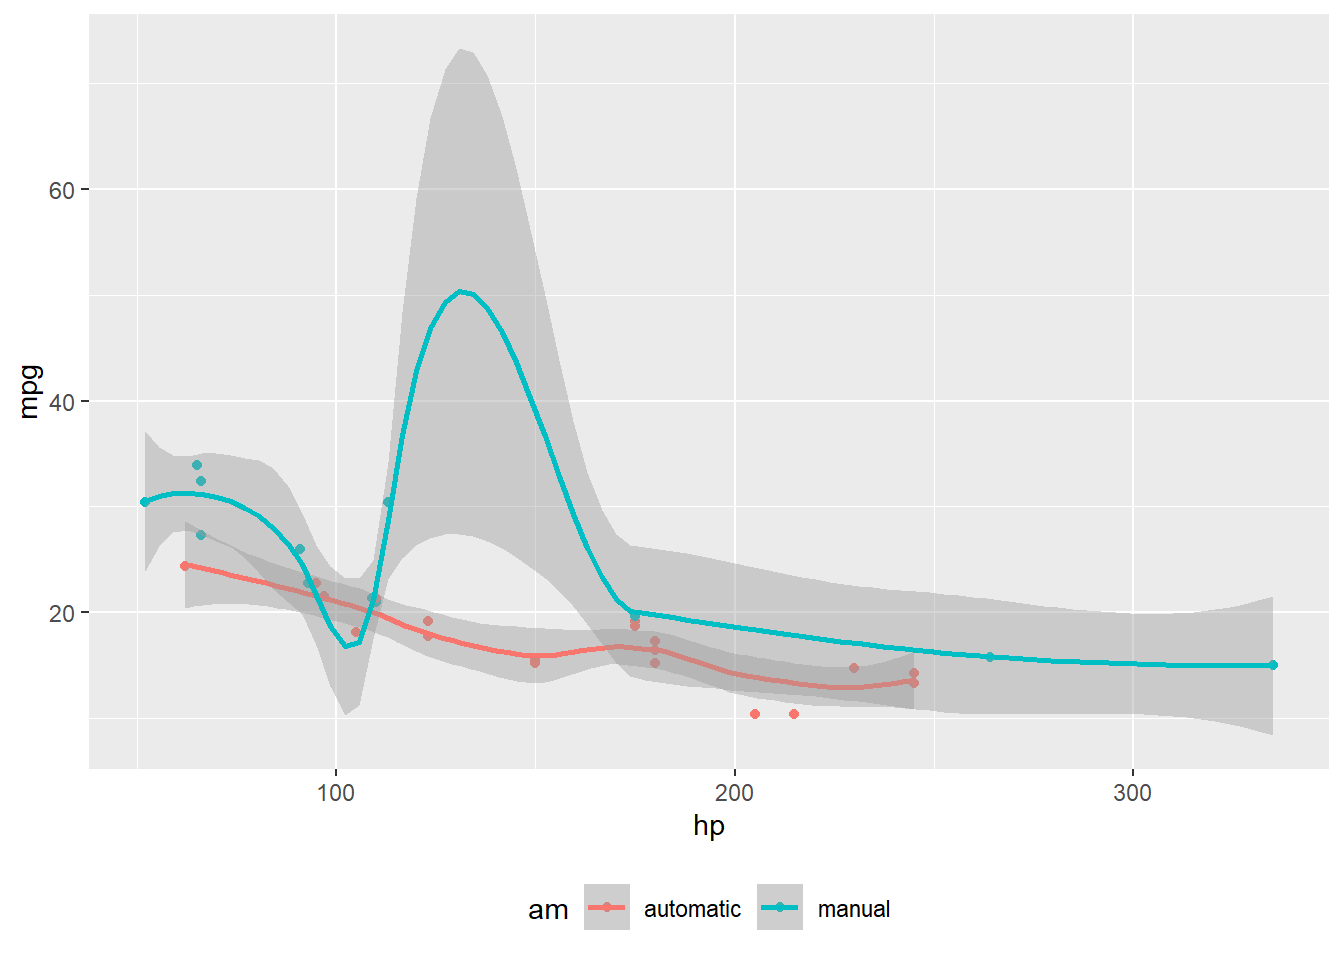
\includegraphics{metodologia_files/figure-latex/unnamed-chunk-1-1.pdf}

Aqui vamos a testear si funciona un gráfico interactivo.

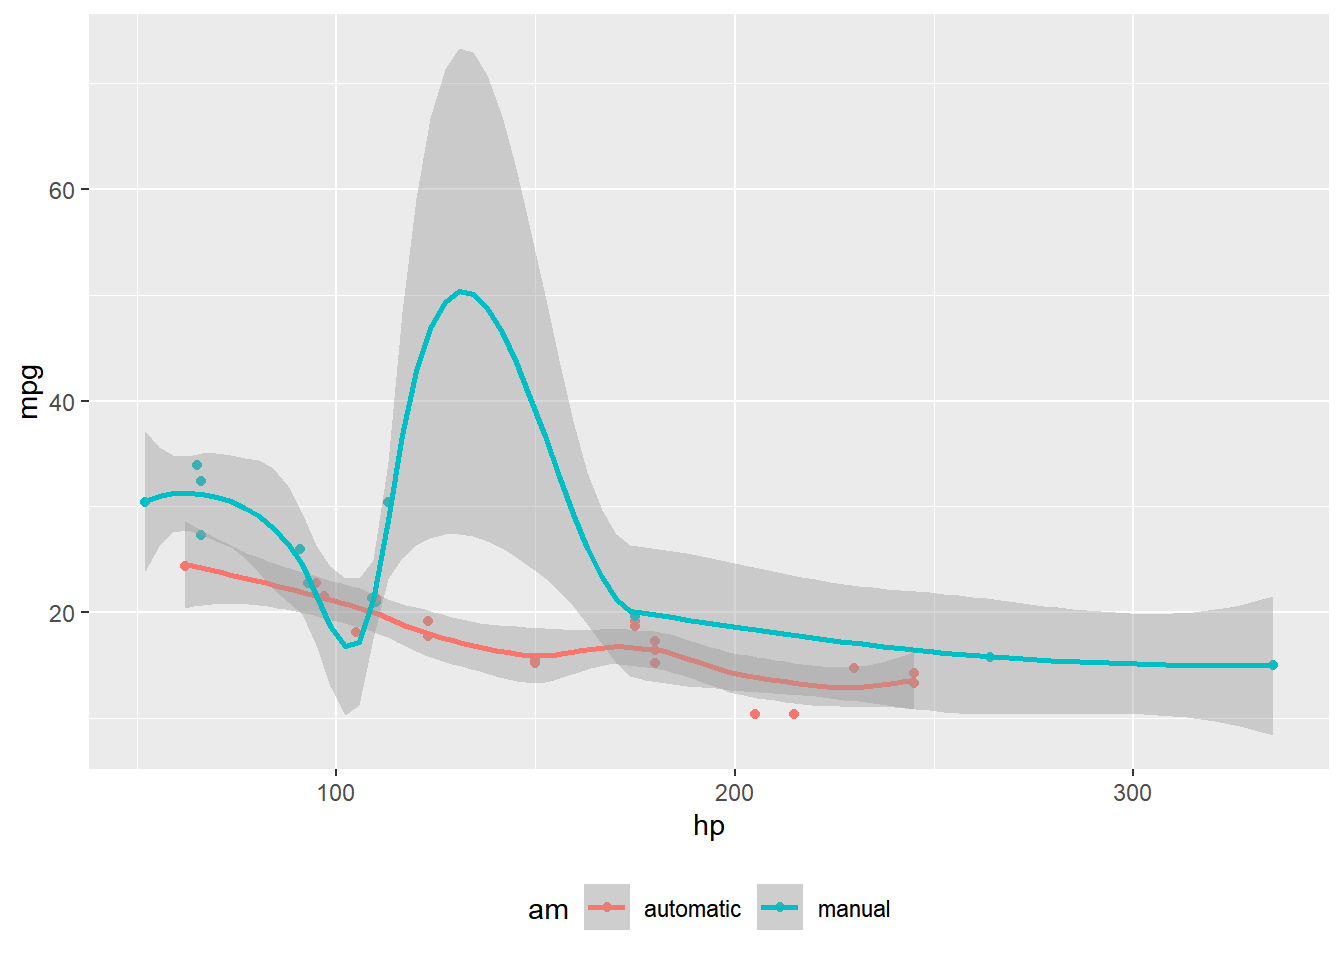
\includegraphics{metodologia_files/figure-latex/unnamed-chunk-3-1.pdf}

\hypertarget{empecemos-por-el-final-el-producto-de-la-investigaciuxf3n.}{%
\chapter{Empecemos por el final: el producto de la investigación.}\label{empecemos-por-el-final-el-producto-de-la-investigaciuxf3n.}}

\hypertarget{ruta}{%
\chapter{Ruta}\label{ruta}}

Cambios de pregunta de investigación

\hypertarget{paradigmas}{%
\chapter{Paradigmas}\label{paradigmas}}

\hypertarget{errores-muxe1s-comunes}{%
\chapter{Errores más comunes}\label{errores-muxe1s-comunes}}

We have finished a nice book.

  \bibliography{book.bib,packages.bib}

\end{document}
